\documentclass[14pt,a4paper,oneside]{extbook}
\usepackage[utf8]{vietnam}
\usepackage{amsmath,amssymb,mathrsfs,fancyhdr,enumerate,multirow,makecell}
\usepackage{tkz-euclide,tikz-3dplot,tikz,tkz-tab}
\usetikzlibrary{arrows.meta,calc,intersections,angles,quotes,backgrounds,shapes.geometric,patterns,through,shadows,positioning}
\usepackage{yhmath}
\usepackage[top=0.7cm, bottom=0.7cm, left=1.0cm, right=1.0cm, headheight=16pt, headsep=3mm, footskip=5mm]{geometry}
\usepackage[hidelinks,unicode]{hyperref}
\usepackage{qrcode}
\usepackage[many]{tcolorbox}
\usepackage{fontawesome}

\pagestyle{fancy}
\fancyhf{}
\fancyhead[L]{\footnotesize\bfseries\color{teal!85!black}\faBook~SỔ TAY KIẾN THỨC TOÁN 5}
\fancyhead[R]{\footnotesize\bfseries\color{blue!85!black}Lớp Toán Thầy Lĩnh -- loptoanthaylinh.vn}
\fancyfoot[C]{\footnotesize\bfseries\color{gray!80!black}-- Sổ tay kiến thức: Bài 15. Ki-lô-mét vuông. Héc-ta --}
\renewcommand{\headrulewidth}{0.4pt}

\begin{document}

% --- BANNER TIÊU ĐỀ BÀI HỌC ---
\noindent
\begin{tcolorbox}[
  enhanced,
  colback=teal!8!white,
  colframe=teal!80!black,
  arc=3mm,
  boxrule=1.1pt,
  width=\linewidth,
  halign=center,
  top=2.2mm, bottom=2.2mm,
  left=3mm, right=3mm,
  drop fuzzy shadow
]
  {\large\bfseries\color{teal!95!black}\faBookmark\ BÀI 15. KI-LÔ-MÉT VUÔNG. HÉC-TA}\\[2pt]
  {\scriptsize\color{black!75}\itshape Đơn vị đo diện tích lớn: Định nghĩa km2, ha, quy đổi và ứng dụng thực tế trên 1 trang A4}
\end{tcolorbox}

\vspace{3.2mm}
% --- KHỐI 1: KHÁI NIỆM KM2 VÀ HÉC-TA ---
\noindent
\begin{minipage}[t]{0.52\textwidth}
  \begin{tcolorbox}[
    enhanced,
    title={\footnotesize\bfseries\color{white}\faMap\ 1. Ki-lô-mét vuông ($\text{km}^2$)},
    colback=blue!2!white,
    colframe=blue!75!black,
    arc=2.5mm, boxrule=0.8pt, top=1.8mm, bottom=1.8mm, left=2.2mm, right=2.2mm
  ]
    \footnotesize
    $\bullet$ Để đo diện tích rất lớn như thành phố, tỉnh, quốc gia, diện tích rừng\dots\\
    $\bullet$ Ki-lô-mét vuông là diện tích của \textbf{hình vuông có cạnh dài $1\text{ km}$}.\\
    \begin{tcolorbox}[colback=white, colframe=blue!75!black, boxrule=0.5pt, arc=1.5mm, halign=center, top=1mm, bottom=1mm]
      {\scriptsize\bfseries\color{blue!90!black}$1\text{ km}^2 = 1\,000\,000\text{ m}^2 = 100\text{ ha}$}
    \end{tcolorbox}
  \end{tcolorbox}
\end{minipage}%
\hfill
\begin{minipage}[t]{0.46\textwidth}
  \begin{tcolorbox}[
    enhanced,
    title={\footnotesize\bfseries\color{white}\faTree\ 2. Héc-ta ($\text{ha}$)},
    colback=teal!2!white,
    colframe=teal!75!black,
    arc=2.5mm, boxrule=0.8pt, top=1.8mm, bottom=1.8mm, left=2mm, right=2mm
  ]
    \footnotesize
    $\bullet$ Thường dùng đo diện tích đất nông nghiệp, lâm nghiệp, đồn điền, trang trại.\\
    $\bullet$ $1\text{ héc-ta}$ là diện tích của \textbf{hình vuông có cạnh dài $100\text{ m}$}.\\
    \begin{tcolorbox}[colback=white, colframe=teal!75!black, boxrule=0.5pt, arc=1.5mm, halign=center, top=1mm, bottom=1mm]
      {\scriptsize\bfseries\color{teal!95!black}$1\text{ ha} = 10\,000\text{ m}^2$} \quad ($1\text{ hm}^2 = 1\text{ ha}$)
    \end{tcolorbox}
  \end{tcolorbox}
\end{minipage}

\vspace{3mm}

% --- KHỐI 2: QUAN HỆ ĐỔI ĐƠN VỊ ---
\noindent
\begin{tcolorbox}[
  enhanced,
  title={\footnotesize\bfseries\color{white}\faExchange\ 3. Mối quan hệ giữa $\text{km}^2$, $\text{ha}$ và $\text{m}^2$},
  colback=purple!2!white,
  colframe=purple!70!black,
  arc=2.5mm, boxrule=0.8pt, top=1.8mm, bottom=1.8mm, left=2.5mm, right=2.5mm
]
  \footnotesize
  \begin{tabular}{ll}
    $\bullet$ $1\text{ km}^2 = 100\text{ ha}$ & $\triangleright$ Đổi từ $\text{km}^2 \rightarrow \text{ha}$: \textbf{Nhân với 100} (VD: $3,5\text{ km}^2 = 350\text{ ha}$).\\
    $\bullet$ $1\text{ ha} = \dfrac{1}{100}\text{ km}^2 = 0,01\text{ km}^2$ & $\triangleright$ Đổi từ $\text{ha} \rightarrow \text{km}^2$: \textbf{Chia cho 100} (VD: $45\text{ ha} = 0,45\text{ km}^2$).\\
    $\bullet$ $1\text{ ha} = 10\,000\text{ m}^2$ & $\triangleright$ $1\text{ m}^2 = \dfrac{1}{10000}\text{ ha} = 0,0001\text{ ha}$.
  \end{tabular}
\end{tcolorbox}

\vspace{3mm}

% --- KHỐI 3: SƠ ĐỒ TƯ DUY ---
\noindent
\begin{tcolorbox}[
  enhanced,
  title={\footnotesize\bfseries\color{white}\faSitemap\ Sơ đồ chuyển đổi ba đơn vị diện tích lớn},
  colback=yellow!2!white,
  colframe=teal!85!black,
  arc=3mm, boxrule=0.9pt, top=1.8mm, bottom=1.8mm, left=1.5mm, right=1.5mm,
  halign=center
]
  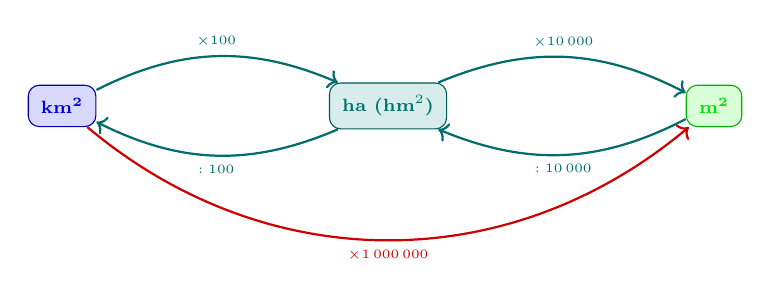
\begin{tikzpicture}[
    scale=0.92,
    every node/.style={transform shape},
    b1/.style={rectangle, rounded corners=4pt, fill=blue!15, draw=blue!70!black, text=blue!90!black, font=\bfseries\scriptsize, inner sep=5pt},
    b2/.style={rectangle, rounded corners=4pt, fill=teal!15, draw=teal!70!black, text=teal!90!black, font=\bfseries\scriptsize, inner sep=5pt},
    b3/.style={rectangle, rounded corners=4pt, fill=green!15, draw=green!70!black, text=green!90!black, font=\bfseries\scriptsize, inner sep=5pt}
  ]
    \node[b1] (km) at (-4.5, 0) {$\mathbf{km^2}$};
    \node[b2] (ha) at (0, 0) {$\mathbf{ha}$ ($\text{hm}^2$)};
    \node[b3] (m) at (4.5, 0) {$\mathbf{m^2}$};

    \draw[teal!85!black, thick, ->] (km) to[bend left=25] node[above, font=\tiny\bfseries] {$\times 100$} (ha);
    \draw[teal!85!black, thick, ->] (ha) to[bend left=25] node[below, font=\tiny\bfseries] {$: 100$} (km);
    \draw[teal!85!black, thick, ->] (ha) to[bend left=25] node[above, font=\tiny\bfseries] {$\times 10\,000$} (m);
    \draw[teal!85!black, thick, ->] (m) to[bend left=25] node[below, font=\tiny\bfseries] {$: 10\,000$} (ha);
    \draw[red!80!black, thick, ->] (km) to[bend right=40] node[below, font=\tiny\bfseries] {$\times 1\,000\,000$} (m);
  \end{tikzpicture}
\end{tcolorbox}

\vspace{3mm}

% --- KHỐI 4: VÍ DỤ ĐỔI SỐ THẬP PHÂN & BẪY TRẮC NGHIỆM ---
\noindent
\begin{minipage}[t]{0.54\textwidth}
  \begin{tcolorbox}[
    enhanced,
    title={\footnotesize\bfseries\color{white}\faBolt\ Viết số đo diện tích dưới dạng số thập phân},
    colback=green!3!white,
    colframe=green!60!black,
    arc=2.5mm, boxrule=0.8pt, top=1.8mm, bottom=1.8mm, left=2.2mm, right=2.2mm
  ]
    \footnotesize
    $\bullet$ $5\text{ km}^2\ 12\text{ ha} = 5\dfrac{12}{100}\text{ km}^2 = 5,12\text{ km}^2$.\\
    $\bullet$ $3\text{ km}^2\ 4\text{ ha} = 3\dfrac{4}{100}\text{ km}^2 = 3,04\text{ km}^2$ (Chú ý số 0!).\\
    $\bullet$ $8\text{ ha}\ 250\text{ m}^2 = 8\dfrac{250}{10000}\text{ ha} = 8,025\text{ ha}$.
  \end{tcolorbox}
\end{minipage}%
\hfill
\begin{minipage}[t]{0.44\textwidth}
  \begin{tcolorbox}[
    enhanced,
    title={\footnotesize\bfseries\color{white}\faExclamationTriangle\ Mẹo tránh bẫy trắc nghiệm},
    colback=red!2!white,
    colframe=red!70!black,
    arc=2.5mm, boxrule=0.8pt, top=1.8mm, bottom=1.8mm, left=2.2mm, right=2.2mm
  ]
    \footnotesize
    $\bullet$ \textbf{Lỗi quên số 0}: $2\text{ km}^2\ 7\text{ ha} \neq 2,7\text{ km}^2$ mà phải là $2,07\text{ km}^2$.\\
    $\bullet$ Nhớ rõ: $1\text{ ha}$ bằng $10\,000\text{ m}^2$ ($4$ chữ số $0$, không phải $100$ hay $1\,000$).
  \end{tcolorbox}
\end{minipage}

\end{document}
